%************************************************
\chapter{Introduction}\label{ch:introduction}
%************************************************

CERN, European Organization for Nuclear Research, (French: Conseil européen
pour la recherche nucléaire) is an European research organization that operates
the largest particle physics laboratory in the world.

Its mission is to: 
\begin{itemize}
	\item Provide a unique range of particle accelerator facilities that enable research at the forefront of human knowledge
	\item Perform world-class research in fundamental physics
	\item Unite people from all over the world to push the frontiers of sciences and technology, for the benefits of all.
\end{itemize}

It host the instrument of the 4 biggest physic collaboration: 
\begin{itemize}
\item ALICE
\item ATLAS
\item CMS
\item LHCb
\end{itemize}

CERN host also a plethora of smaller physical collaborations that benefits from
the instruments, know how, network effect and services availables.

Between the services offered to its users the computing service is one of the
most interesting. Indeed CERN host and manage one of the biggest computing
data center used for public research.

An issues that affect the operations inside the data center is the provisioning
of software on the computing servers.

A specialization of the same problem is the provisioning of containers images.

The general problem of software provisioning is been solved by the use of
CVMFS, a read only file-system that provides a scalable, reliable and low
maintenance software distribution system.

This thesis will explore the problem of creating a suitable read-only
file-system structure to provision containers images on computing nodes. We
will provide a general read-only file-system structure and we will implement the
proposed methodology on top of CVMFS.

This thesis is composed by several parts: The background will provide the
necessary information on the CERN computing architecture (WLCG), then we will
explore CVMFS and why it is a good fit for the CERN computing architecture, the
last part of the background will cover the integration between CVMFS and
containers technologies.  The state of the art will explore what alternatives
are available for software distribution in general and for distribution of
images.  We will then define the problem that this thesis is trying to solve
and few metrics of interest in our specific case.  The methodology part will
explain the details of the solution we propose for this specific problem.  The
implementation chapter will focus on how the proposed methodology is been put
in practise.  We will evaluate the result of the proposed methodology and
implementation on the result part following the metrics that were previously
proposed.  Finally we will propose future work and enhancement to the
implementation

\chapter{Background}\label{ch:background}

In this chapter we are going to introduce the concept and technologies that
made this work possible.  We will start introducing the Worldwide LHC Computing
Grid (WLCG) which is the collaboration that provide the computing power
necessary to the CERN mission. The dimension of the WLCG and its specific
workload required and allowed a specific software distribution system,
CernVM-FileSystem which is used to provision the machine on the WLCG.

Then we will introduce the concept of containers a different way to solve the
software distribution problem widely adopted in the industry. In particular we
will focus on Docker containers and the Docker images format. We will then
explore Singularity, in which we are mostly interested in its capability to run
containers whose content is all already unpacked in a simple directory. Finally
we will explore the Docker \texttt{cvmfs/graphdriver}, a Docker plugins that
allow to run Docker images whose content is available on a read-only
file-system without the need of downloading or access the Docker standard
images.


\section{WLCG}

The Worldwide LHC Computing Grid is an global collaboration of more than 170
data centers in 42 countries.  The mission of the WLCG is to provide the
computing resource to store, distribute and analyze the data from the operation
of the LHC.

The organization of the WLCG follow a hierarchical model, where each level is
called “Tier” The most central Tier is the Tier-0 hosted by CERN in the Geneva
Area and in Budapest. There are 13 Tier-1 data center with enough storage and
computing capabilities to support the Grid operation around the clock, the
Tier-1 are connected to the Tier-0 with at least 10Gb/sec links.  Tiers-1 are
geographically distributed, 8 of them are in Europe, 3 in the North American
and the rest in Asia. Finally the Tier-2 data center do not have strict
requirements and are generally operated by research centers and universities.

\begin{figure}
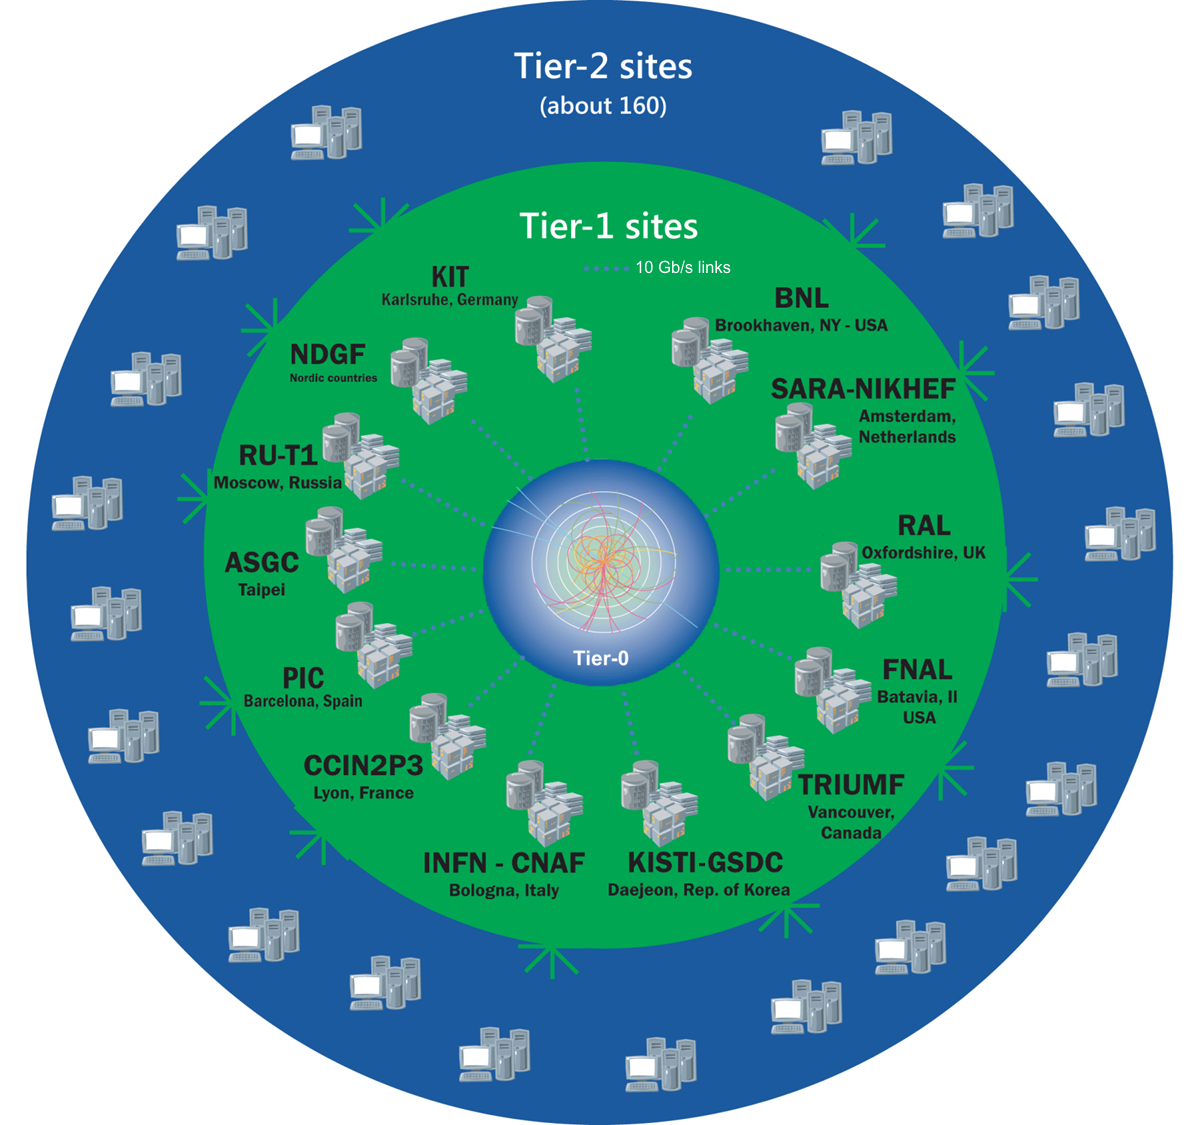
\includegraphics[width=\textwidth,height=\textheight,keepaspectratio]{gfx/WLCG}
\caption{Schematic representation of the WLCG}
\label{fig:wlcg-schema}
\end{figure}

A schematic representation of the architecture of the WLCG is provide on figure
\ref{fig:wlcg-schema}.


The work on the WLCG is mostly divided in two big classes: analysis of the data
from the LHC detectors and Monte Carlo simulations.  The WLCG assume and
support a batch computing paradigm. Analysis and simulations are split in
smaller jobs that are distributed to different computing node that can work in
parallel.

Before to start each job it is necessary to install the software on the server.
Unfortunately the amount of software potentially needed in each computing node
and the velocity at which the software is updated makes the installation
challenging. Moreover simpler installation techniques that relies on packages
managers are not applicable since they would put the package managers
themselves under too much load.

Several solution have been proposed and used, but eventually it settled for the
use of CernVM-FileSystem (CVMFS).

\section{CVMFS}

This section will explore CernVM-FileSystem, we will start with an high level
overview of CVMFS, then we will explore what happens when a file is requested.

% need to really talk about the sub-catalog system

\subsection{CVMFS High Level Overview}

CernVM-FileSystem provides a scalable, reliable and low-maintenance software
distribution system. It is implemented as a read-only POSIX file-system in user
space exploiting FUSE (File-system in USErspace) and standard web server
technologies such as Apache or NGNIX.

CVMFS organize its content in repositories where we can approximate each
repository as a CVMFS instance.

CVMFS is engineered to support repository of size on the order of the Terabyte
with billions of files.

To save storage space files are addressed by their content (Content Addressable
Storage), hence duplicated files will be stored only once.

In order to distribute software to geographically distant data centers and keep
a low latency, CVMFS allows to cache content in different machines. This allow
to host a cache server in each Tier of the WLCG. The use of caches fits
perfectly with the Tiers models of the WLCG presented above. The Tier-0 host
the main repository (Stratum-0), and the Tier-1 host the first level of cache
(Stratum-1) and so on.

The content of the files are served using the HTTP protocol by a standard
web server. The files are lazily downloaded only on the machine that need them
and only when necessary.

In order to locate and request files from CVMFS the clients download the
catalog a simple SQLite database which describes a subtree of the whole
file-system.  The catalog contains all the metadata of files and directories,
including owner, group, permission, and size. Moreover the catalog contains
also the URL where to download the files.

A root catalog is available in a know path, and, if the file-system grows too
large, the root catalog links to other sub-catalogs. The use of sub-catalogs
allows to keep each catalog small improving the query time.

\subsection{CVMFS Details}

CVMFS is implemented using the Client-Server architecture. The server is
responsible to manage the content of the repository and expose it via HTTP API.
The client is installed in the host machine and is responsible to expose the
content of the repository to the users. The client is implemented as a FUSE
daemon which implements all the system calls necessary for a read-only
file-system. 

When a CVMFS file-system is mounted, it start by reading a configuration file
which describe each repository. The client then download a simple file text
file which point to the catalog of the repository. Once the catalog is
downloaded the client has all the information necessary to start responding to
the system call from the user.

As an example, when the user requires a \texttt{stat} system call against a
file the client reads from the catalog all the information about the file like,
size, permission, mode, etc.. and reply    with them.

When the user require to read from a file, then the client first download the
file from the server, store it into a local cache and pass through each read
operation to the local copy.

This approach allow to download only the file really required, since all the
other system calls can be served only by reading from the catalog. However it
implies that the reading latency from a file depends on the network latency.

This approach works very well if the reading latency of a file is not a major
concern and if reading from the catalog is fast. However, if the catalog grow
too big, then the queries become too slow, to overcome this problem the
sub-catalogs were introduced.

A sub-catalog is exactly like the normal catalog but while the catalog refers
to the whole file-system tree, a sub-catalog refer to a smaller sub tree of the
file-system. In order to avoid confusion, we will refer to the root-catalog as
the catalog which include the root of the file-system and to sub-catalog to all
the other catalogs in the file-system. The root-catalog, of course, embed
several sub-catalogs, and each sub-catalog can, recursively, embed another
sub-catalog.

When is required to read information about a file the client start by looking
into the root catalog and then follows the sub-catalog structure until it does
not find the required file.

\section{Containers}

While CERN solved its problems of software distribution with CVMFS the industry
opted for a different approach, containers.

Containers are a standard unit of software that packages up code and all its
dependencies so that computer applications run quickly and reliable from one
computing environment to the others.

The containers are packed up in a specific format, in this work we are only
interested in the format used by Docker, called Docker images defined in the
OCI standard. A Docker image is an immutable set of tar files, each tar file is
called a layer. Before to run the container each layer get mounted one on top
of the other to re-create the original environment where to run the
application. The content of each image is codified in a \texttt{json} file, the
manifest, which provide the unique name of the image itself and which refer to
each layer that compose the image by their unique identifiers. The unique
identifier of both images and layers is the result of the function
\texttt{hash256} of their content.

Docker images are distributed through Docker registries, simple HTTP servers
that given the unique identifiers of a layer provides the layer itself,
similarly, given the identifier of an image the registries provides its
manifest.

Docker allow to associate a human readable identifier to each image, this name
is composed by a namespace, which identify the user or organization that create
the image, a name, which identify the image itself and a tag, which identify
the version of the image. These names are not immutable and are meant to be
used just by humans to reason about the images.

The repository where the image is hosted, its namespace, its name and its tag
create a hierarchical structure between the several images that is easy to
navigate for humans.

\subsection{Docker and the cvmfs/graphdriver plugin}
\label{subsec:docker-thin-images}

Docker is a thin CLI layer on top of a Linux daemon, \texttt{dockerd} which is
responsible to obtains the Docker images from the registries, mount the layers,
manage the runtime of the image and allow communication of a Docker runtime
with the host system.

Docker layers can be shared between different images, so the Docker daemon
download them once and store them in the local machine for future use. On
average only 7\% of the content inside a Docker images is used during the
runtime of the image. The layers are distributed as a single tar file, hence a
naive distribution of layers with CVMFS would not provide any advantage. The
whole tar files would need to be downloaded erasing the advantages of using
CVMFS.

A solution to this problem was introduced with the \texttt{cvmfs/graphdriver}
plugin and the concept of "thin-images". In this work we are not interested in
the internal of the \texttt{cvmfs/graphdriver} plugin, it will be sufficient to
know that the Docker daemon can be enhance with the use of plugins and that the
plugin allows us to run what are called "thin-images".

"Thin-images" are Docker images that are created starting from a standar
("fat") Docker images. The content of a "thin-image" is only a simple
\texttt{json} file whose content is the layers needed by the original
"fat-image" and where to find them in the host file-system, we call this file
the "recipe". "Thin-images" can be executed only if the Docker daemon have
enable the \texttt{cvmfs/graphdriver} plugin, indeed the plugin is able to read
the content of the thin-image, mount the original layers inside the container,
and finally execute the application.

If the files necessary to run the "thin-images" are distributed by CVMFS is
possible to run docker containers without downloading any unnecessary content.

Moreover the \texttt{cvmfs/graphdriver} plugin is able to run standard ("fat") Docker images, hence is possible to enable the plugin and forget about having it. 

On figure \ref{fig:flowchart-run-thin-image} we show how the plugin run a Docker image. 

\begin{figure}
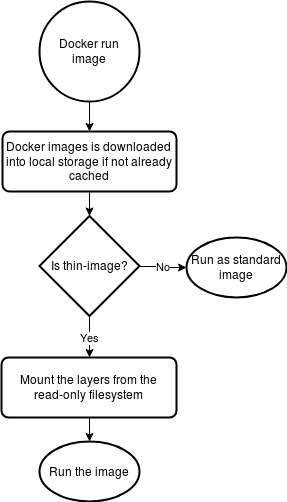
\includegraphics{gfx/RunThinImages}
\caption{Decision proces for running docker thin images}
\label{fig:flowchart-run-thin-image}
\end{figure}

A problem with this approach is that a "thin-image" can be downloaded, store in
the local storage and successfully run using the content provide by CVMFS. On a
second moment the images can be update, uploaded newly on the registry and the
old content in CVMFS is deleted to host the new content of the image. If now
the user try to run the same images, it will not download it again from the
registry but it will use the image already cached, this thin-image will refer
to content not available anymore on CVMFS, hence it will fail to run.

\subsection{Singularity}

Singularity is another container runtime, it provides its own image format but
is capable to run standard Docker images as well. Moreover is capable of
running containers, also Docker containers, directly from a directory
containing the unpacked container file-system itself. 

Given the Singularity capability to run Docker containers directly from a
directory containing the unpacked Docker image file-system its integration with
CVMFS is simpler that the one with Docker itself. Indeed is sufficient to host
the directory containing the unpacked file-system of the Docker image in CVMFS.


